\documentclass[paper=letter,11pt]{scrartcl}

\KOMAoptions{headinclude=true, footinclude=false}
\KOMAoptions{DIV=14, BCOR=5mm}
\KOMAoptions{numbers=noendperiod}
\KOMAoptions{parskip=half}
\addtokomafont{disposition}{\rmfamily}
\addtokomafont{part}{\LARGE}
\addtokomafont{descriptionlabel}{\rmfamily}
%\setkomafont{pageheadfoot}{\normalsize\sffamily}
\setkomafont{pagehead}{\normalsize\rmfamily}
%\setkomafont{publishers}{\normalsize\rmfamily}
\setkomafont{caption}{\normalfont\small}
\setcapindent{0pt}
\deffootnote[1em]{1em}{1em}{\textsuperscript{\thefootnotemark}\ }


\usepackage{amsmath}
\usepackage[varg]{txfonts}
\usepackage[T1]{fontenc}
\usepackage{graphicx}
\usepackage{xcolor}
\usepackage[american]{babel}
% hyperref is needed in many places, so include it here
\usepackage{hyperref}

\usepackage{xspace}
\usepackage{multirow}
\usepackage{float}


\usepackage{braket}
\usepackage{bbm}
\usepackage{relsize}
\usepackage{tcolorbox}

\def\ketY{\ensuremath{\ket {\Psi}}}
\def\iGeV{\ensuremath{\textrm{GeV}^{-1}}}
%\def\mp{\ensuremath{m_{\textrm{proton}}}}
\def\rp{\ensuremath{r_{\textrm{proton}}}}
\def\me{\ensuremath{m_{\textrm{electron}}}}
\def\aG{\ensuremath{\alpha_G}}
\def\rAtom{\ensuremath{r_{\textrm{atom}}}}
\def\rNucl{\ensuremath{r_{\textrm{nucleus}}}}
\def\GN{\ensuremath{\textrm{G}_\textrm{N}}}
\def\ketX{\ensuremath{\ket{\vec{x}}}}
\def\ve{\ensuremath{\vec{\epsilon}}}


\def\ABCDMatrix{\ensuremath{\begin{pmatrix} A &  B  \\ C  & D \end{pmatrix}}}
\def\xyprime{\ensuremath{\begin{pmatrix} x' \\ y' \end{pmatrix}}}
\def\xyprimeT{\ensuremath{\begin{pmatrix} x' &  y' \end{pmatrix}}}
\def\xy{\ensuremath{\begin{pmatrix} x \\ y \end{pmatrix}}}
\def\xyT{\ensuremath{\begin{pmatrix} x & y \end{pmatrix}}}

\def\IMatrix{\ensuremath{\begin{pmatrix} 0 &  1  \\ -1  & 0 \end{pmatrix}}}
\def\IBoostMatrix{\ensuremath{\begin{pmatrix} 0 &  1  \\ 1  & 0 \end{pmatrix}}}
\def\JThree{\ensuremath{\begin{pmatrix}    0 & -i & 0  \\ i & 0  & 0 \\ 0 & 0 & 0 \end{pmatrix}}} 
\def\JTwo{\ensuremath{\begin{bmatrix}    0 & 0 & -i  \\ 0 & 0  & 0 \\ i & 0 & 0 \end{bmatrix}}}
\def\JOne{\ensuremath{\begin{bmatrix}    0 & 0 & 0  \\ 0 & 0  & -i \\ 0 & i & 0 \end{bmatrix}}}
\def\etamn{\ensuremath{\eta_{\mu\nu}}}
\def\Lmn{\ensuremath{\Lambda^\mu_\nu}}
\def\dmn{\ensuremath{\delta^\mu_\nu}}
\def\wmn{\ensuremath{\omega^\mu_\nu}}
\def\be{\begin{equation*}}
\def\ee{\end{equation*}}
\def\bea{\begin{eqnarray*}}
\def\eea{\end{eqnarray*}}
\def\bi{\begin{itemize}}
\def\ei{\end{itemize}}
\def\fmn{\ensuremath{F_{\mu\nu}}}
\def\fMN{\ensuremath{F^{\mu\nu}}}
\def\bc{\begin{center}}
\def\ec{\end{center}}
\def\nus{$\nu$s}

\def\adagger{\ensuremath{a_{p\sigma}^\dagger}}
\def\lineacross{\noindent\rule{\textwidth}{1pt}}

\newcommand{\multiline}[1] {
\begin{tabular} {|l}
#1
\end{tabular}
}

\newcommand{\multilineNoLine}[1] {
\begin{tabular} {l}
#1
\end{tabular}
}



\newcommand{\lineTwo}[2] {
\begin{tabular} {|l}
#1 \\
#2
\end{tabular}
}

\newcommand{\rmt}[1] {
\textrm{#1}
}


%
% Units
%
\def\m{\ensuremath{\rmt{m}}}
\def\GeV{\ensuremath{\rmt{GeV}}}
\def\pt{\ensuremath{p_\rmt{T}}}


\def\parity{\ensuremath{\mathcal{P}}}

\usepackage{cancel}
\usepackage{ mathrsfs }
\def\bigL{\ensuremath{\mathscr{L}}}

\usepackage{ dsfont }



\usepackage{fancyhdr}
\fancyhf{}


\lhead{\Large 33-444} % \hfill Introduction to Particle Physics \hfill Spring 2019}
\chead{\Large Introduction to Particle Physics} % \hfill Spring 2019}
\rhead{\Large Spring 2022} % \hfill Introduction to Particle Physics \hfill Spring 2019}
\begin{document}
\thispagestyle{fancy}





%\begin{tabular}{c}
%{\large 33-444 \hfill Intro To Particle \hfill Spring 2019\\}
%\hline 
%\end{tabular}

\begin{center}
{\huge \textbf{Midterm 2}}
\large

\end{center}

{\large


\textbf{1) List or draw a diagram of the particles in the Standard model. } \hfill \textit{(6 points)}\\
What is the spin of each particle ?

\vspace*{3.5in}


\textbf{2) Why is the weak interaction so much weaker than then electromagnetic interactions at low energies?} \hfill \textit{(2 points)}\\

\vspace*{0.5in}

\clearpage

\textbf{3) Feynman Diagrams }\hfill \textit{(12 points)}\\
Fermions of type $x$ scatter into fermions of type $y$ through the diagram shown below, where $S$ is a massive scalar. 
At low energies ($P_x P_y << m_S$) the cross section for this process is given by $\sigma_0$.
Assume $m_x$ and $m_y$ are both negligible.
\bc
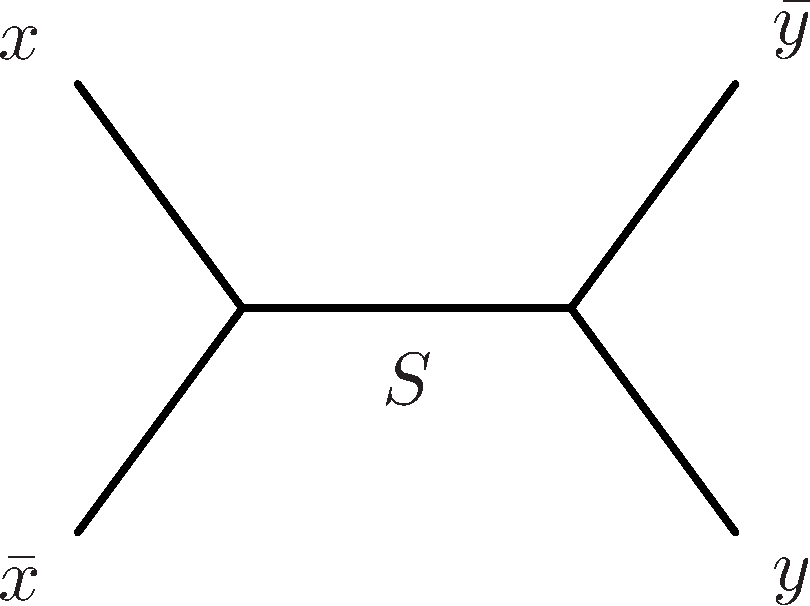
\includegraphics[width=0.2\textwidth]{./xxToyy.pdf}
\ec
\bi
\item[a)] How does this cross section change if the ``S-charge'' of the $x$ particle is doubled ? \\ (S-charge being the $x\bar{x} \rightarrow S$ coupling) 
\vspace*{1.5in}
\item[b)] How does the cross section change if the mass of the $S$-particle is doubled ?
\vspace*{1.5in}
\item[c)] At low energies, how does the cross section depend on the center of mass energy of the scattering $E_{CM}$ ? 
\textit{(Hint: At low energies you can think of the $xx \rightarrow yy$ scattering as described by an effective 4-point $xxyy$ interaction, as Fermi did for neutrino scattering.)}
\ei

\clearpage

\textbf{4) Di-boson physics:  } \hfill \textit{(6 points)}\\
Processes in which pairs of gauge bosons are produced are a sensitive probe of the electro-weak theory. These are typically studied at the LHC by looking for signatures involving electrons or muons.  
Estimate how often a $WZ$ event decays into an electron or muon and three neutrinos.\\ ie: $e\nu\nu\nu$ or $\mu\nu\nu\nu$

\vspace{4.in}

%\textbf{4) Higgs Boson discovery: } \hfill \textit{(5 points)}\\
%The Higgs boson was discovered in its decays to $WW (Br\sim20\%)$, $ZZ\ (Br\sim3\%)$ and $\gamma\gamma\ (Br\sim0.2\%)$.
%However for the $WW$ and $ZZ$ decays, only the ``fully-leptonic'' channels -- where each boson decays leptonicically to $e$ or $\mu$ -- were used. \\
%
%Estimate how often $WW \rightarrow \ell\nu\ell'\nu'$ and $ZZ\rightarrow\ell\ell\ell'\ell'$, where $\ell$ is e or $\mu$. (ignore decays through taus)\\
%
%Including these factors, rank the Higgs boson discovery channels by how many signal events they are expected to have.
%
%\vspace{0.5in}

%\textbf{5) Accelerators: } \hfill \textit{(4 points)}\\
%\begin{itemize}
%\item[a)]{What limits the energy of circular proton accelerators ?
%}
%\item[b)]{What limits the energy of circular electron accelerators ?
%}
%\end{itemize}
%

%\textbf{6) Electron-positron Collisions } \hfill \textit{(6 points)}\\
%\begin{itemize}
%\item[a)]{
%How does the value of $R(E_{CM}) \equiv \sigma(ee\rightarrow \rmt{jets})/\sigma(ee\rightarrow \mu\mu)$ change as $E_{CM}$ is increased beyond twice the mass of the charm quark? 
%What values of $R(< 2 m_{\rmt{charm}})$ and $R(> 2 m_{\rmt{charm}})$ do you expect?
%}
%
%\item[b)]{Sketch a graph of the total cross section of $ee\rightarrow\mu\mu$ as a function of $E_{CM}$ from 40 GeV to 200. 
%Also sketch the component of the cross section due to the electro-magnetic interaction.
%}
%\end{itemize}


\textbf{5) Collider Detectors  } \hfill \textit{(4 points)}\\
\begin{itemize}
\item[a)]{ In what ways do the detector signatures of electrons and muons look a-like, in what ways are they different ?
}
\vspace*{1.5in}

\item[b)]{ In what ways do the detector signatures of electrons and photons look a-like, in what ways are they different ?
}
\end{itemize}

\clearpage
        

\textbf{6) Calorimeters } \hfill \textit{(4 points)}\\
Hadronic showers or electro-magnetic showers: which are more challenging to accurately measure and why ? 

\vspace*{2.5in}

\textbf{7) For a new particle X with mass $\sim$ 2 TeV,  would you expect to measure the X mass more precisely from $X\rightarrow ee$ or $X \rightarrow \mu\mu$ ? Justify your answer.} \hfill \textit{(4 points)}\\
\vspace*{2.5in}


\textbf{8) How are \nus\ detected at the LHC ?} \hfill \textit{(2 points)}\\


\clearpage

\textbf{9) The God Particle } \hfill \textit{(4 points)} \\ 
Critique the statement:  ``The Higgs Boson (or god particle) is responsible for all the mass in the Universe''

\vspace*{1.5in}

\textbf{10) Higgs Boson Production : } \hfill \textit{(4 points)}\\
Why is Higgs boson production so much rarer then W or Z production despite the fact that their masses are similar?    

\vspace*{1.5in}


\textbf{11) Higgs-Lepton interactions } \hfill \textit{(4 points)}\\
The coupling of the Higgs field to leptons can be studied by looking for detector signals where the Higgs boson decays to pairs leptons.
Which of the possible decay modes would be the best way to do this.  Justify your answer.

\clearpage

\textbf{12) Interaction Symmetries } \hfill \textit{(9 points)} \\ 
In the first part of the course we learned that the interactions of mass-less spin-1 particles must be described by group symmetries. 
\begin{itemize}
\item[a)]{How is the group symmetry of an underlying interaction related to the particle content ?}
\vspace*{1.5in}
\item[b)]{What are the symmetry groups of the electro-weak interaction in the SM ? }
\vspace*{1.5in}
\item[c)]{How does the observed physical particle content in the SM reflect this ? (Qualitatively, no formulas required.) }
\vspace*{1.5in}
\end{itemize}

%\textbf{14) Spontaneous Symmetry Breaking} \hfill \textit{(6 points)} \\ 
%\begin{itemize}
%\item[a)]{What is Spontaneous Symmetry Breaking  ?  }
%\item[b)]{What properties of the fundamental particles is it responsible for describing ?}
%\item[c)]{What experimental evidence do we have that spontaneous symmetry breaking is actually responsible for these properties?}
%\end{itemize}




} % Begning Large
\end{document}
